\documentclass[a4paper]{article}
\usepackage{tikz}
\usepackage{amsmath,amsthm,amssymb}
\usetikzlibrary{arrows,positioning, calc} 
\tikzstyle{vertex}=[draw,circle,minimum size=20pt,inner sep=0pt]

\begin{document}

\textbf{CSCI 303 -- PS5 \hfill Name: Nathan C. Owen}
~\\\\\

\textit{Exercise 4.1.3}\\
The maximum number of edges in an undirected graph with V vertices is $V(V-1)/2$ edges, and the minimum number of edges of a connected graph with V vertices is $V-1$ edges.
\\

\textit{Exercise 4.2.1}\\
Similarly, in a directed graph, there may be two edges in opposite directions for every non directed edge in an undirected graph. This tells us that that maximum number of edges in a directed graph with V vertices is $V(V-1$, and the minimum number of edges such that no vertex is isolated is still $V-1$.
\\

\textit{Exercise 4.1.10}\\
It is known that every connected graph has a minimum spanning tree, and removing a leaf, better defined as a vertex with only one edge, from this tree will retain the connectivity of the graph. Because such a tree will always exist, and there is at least one leaf in every tree, we can always find such a vertex. To locate a vertex that only has one edge, we can use depth first search to traverse a tree that will choose the very first vertex that has no children, that is a vertex that has no edges other than the edge that was traveled to arrive at this vertex. An example that cares for cycles is below:
\begin{verbatim}
findLeaf(Node):
   visited = true
   if children(Node) == 0
      return Node
   for child in children(Node)
      if isVisited(child)
         continue
      leaf = findLeaf(Child)
      if leaf != Null
         return leaf
   return Null
\end{verbatim}
\textit{Exercise 4.1.12}\\
Because regarding the breadth first search tree we know that the path found from the root to any vertex is guaranteed to be a shortest path, it also follows that for any vertices $v$ and $w$ not at the root that the path between these vertices is guaranteed to be the shortest path that includes the root. Furthermore, if the path from $v$ to $w$ in the BFS tree is a subpath of either the root to $v$ or the root to $w$, then we know that this path is indeed a shortest path from $v$ to $w$.
\\

\textit{Exercise 4.2.11}\\
One family of sparse digraphs whose number of directed cycles grows exponentially in the number of vertices are an augmented form of balanced binary trees, where every edge works in both directions. The addition of bi-directional edges to the leafs of such a graph introduces cycles at a exponential rate. An illustration of one such graph follows.
\\\\\\\\\\\\\\\\\\\\\\

\textit{Exercise 4.3.3}
For contradiction, assume that there exist two minimum spanning trees for a graph in which all edges have distinct weights. Observe an edge $e$ of minimum weight that only exists in one of the MSTs (such a path exists because the MSTs are distinct). Assume the edge exists in the first MST: if this edge is added to the second, it will create a cycle. There is some edge in this second MST that does not exist in the first MST, else the first MST would contain a cycle as well - this edge must be greater than $e$ by our assumption that $e$ was of minimum weight and weights must be distinct. Therefore the second MST is not an MST at all, which is a contradiction. 
\\\\
\textit{Exercise 4.3.4}\\
For counter example, observe this minimum spanning tree in which all edges are of identical weight.





\begin{center}
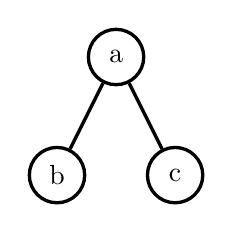
\begin{tikzpicture}[very thick,level/.style={sibling distance=15mm/#1}]
\node [vertex] (a){a}{
  child {
    node [vertex] (b) {b}
    }
  child {
    node [vertex] (c) {c}
  }
  };
\end{tikzpicture}
\end{center}





\end{document}